\documentclass[11pt,a4paper]{article}

% 패키지
\usepackage[left=2cm,right=2cm,top=2cm,bottom=2cm]{geometry}
\usepackage[utf8]{inputenc}
\usepackage[T1]{fontenc}
\usepackage{lmodern}
\usepackage{kotex}      % 한글 폰트
\usepackage{titlesec}
\usepackage{enumitem}
\usepackage{tabularx}
\usepackage{xcolor}
\usepackage{hyperref}
\usepackage{graphicx}
\usepackage{ragged2e}
\usepackage{amsmath}

% 색상 정의
\definecolor{sectioncolor}{RGB}{0, 0, 0}
\definecolor{sungkyungreen}{RGB}{104, 179, 27} % 성균관 로고 초록색

% 섹션 스타일 설정
\titleformat{\section}
  {\Large\bfseries\color{sectioncolor}}
  {}{0em}{}[{\color{sungkyungreen}\titlerule}]
\titlespacing{\section}{0pt}{12pt}{8pt}

% 하이퍼링크 설정
\hypersetup{
    colorlinks=true,
    linkcolor=blue,
    filecolor=blue,
    urlcolor=blue,
}

% 글머리 기호 설정
\setlist[itemize]{label={\scriptsize\raisebox{1pt}{$\bullet$}}}

% 문서 시작
\begin{document}

% 업데이트 날짜 (우측 상단)
\hfill \text{Updated: \today} % \today는 현재 날짜
\vspace{1em} % 날짜와 내용 사이 간격

% 헤더: 이름 및 연락처 정보
\noindent
\begin{minipage}{0.25\textwidth}
    \begin{flushleft}
        % 사진 삽입
        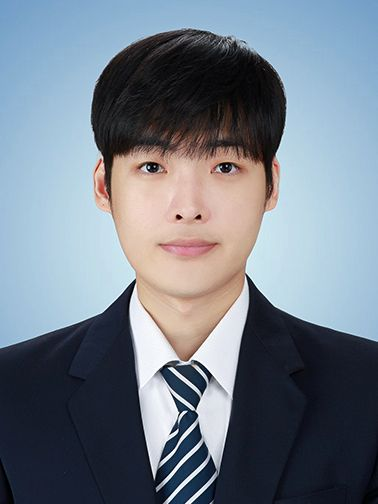
\includegraphics[width=3.5cm]{image/hk.jpg}
    \end{flushleft}
\end{minipage}
\begin{minipage}{0.7\textwidth}
    {\LARGE\textbf{Lee Hakkyu}}\\[5pt]
    {\large {\color{sungkyungreen}\textbf{|}} Sungkyunkwan University}\\[10pt]
    
    \vspace{0.5cm}
    \textbf{EMAIL:} \href{mailto:dir9555@naver.com}{dir9555@naver.com
}\\
    \textbf{Phone:} +82) 010-7599-2509\\
    \textbf{Github:} \href{https://github.com/nakba888}{https://github.com/nakba888}\\
    
\end{minipage}

% 교육
\section{{\color{sungkyungreen}EDU}CATION}

\noindent
\begin{tabularx}{\textwidth}{@{}p{3.5cm}X@{} >{\RaggedLeft}p{3cm}@{}}
Mar.2025 $\sim$  & \textbf{Sungkyunkwan University} & Suwon,\\
Present & Department of Smart Factory & Korea\\
% 한 행 공백 추가
\vspace{5pt}
& Bachelor's Degree Program &\\
& GPA:  3.5 / 4.5  &
\end{tabularx}

% 연구 관심사
\section{{\color{sungkyungreen}RES}EARCH INTERESTS}
\begin{itemize}[leftmargin=*]
    \item Computer vision
    \item Face recognition
\end{itemize}

% 연구 경험
\section{{\color{sungkyungreen}RES}EARCH EXPERIENCES}
\begin{itemize}[leftmargin=*]
    \item Conducted research on deep learning-based facial recognition, including face detection, alignment, and feature embedding extraction., Sungkyunkwan University, Korea (Mar. 2024 $\sim$ Jun. 2024)
\end{itemize}



% 수상 내역
\section{{\color{sungkyungreen}AWA}RDS AND HONORS}
\begin{itemize}[leftmargin=*]
    \item Bronze Award, WCRC Logistics Robot Competition, University Category, Korea (Nov. 2023)
    \item Grand Prize, Startup Idea Competition through Big Data Analysis, University of Seoul, Korea (Jan. 2024)
\end{itemize}

% 프로젝트
\section{{\color{sungkyungreen}PRO}JECTS}
\begin{itemize}[leftmargin=*]
    \item Real-Time Lightweight Facial Recognition System Utilizing YOLO-EdgeFace, Smart Factory Capstone Design, Sungkyunkwan University, Korea (Mar. 2024 ∼ Jun. 2024)
\end{itemize}

% 기술 및 도구
\section{{\color{sungkyungreen}SKI}LLS AND TECHNIQUES}
\begin{itemize}[leftmargin=*]
    \item Python (PyTorch, Tensorflow)
    \item Flutter (Dart) 
    \item C++ (Object-oriented and functional programming)
    \item Image and video processing using OpenCV, PIL, and MTCNN
\end{itemize}

\end{document}
